\documentclass[12pt]{article}

\usepackage{sbc-template}
\usepackage[utf8]{inputenc}
\usepackage{graphicx,url}
\usepackage[brazil]{babel}   
\usepackage[latin1]{inputenc}  
\sloppy

\title{Estrutura conceitual do Modelo para Agentes Normativos}

\begin{document} 

\section{Objetivo}

O modelo proposto tem como por finalidade representar atividades onde um grupo de pessoas  devem atuar de forma colaborativa com o propósito de resolver um problema. Esse problema pode ser dividido em etapas menores conhecidas como objetivos. Essas pessoas podem se relacionar entre sí, podem se relacionar com os artefatos presentes no meio 
onde elas atuam. Os artefatos também possuem a capacidade de se relacionar. Cada objetivo é concluído apenas se  um ou mais relacionamentos forem realizados. A conclusão do objetivo também é função de certos agentes e artefatos que devem ser presentes. 

Outra finalidade do modelo consiste em representar condições que devem ser mantidas ao longo da atividade, se essas condições forem desfeitas - a atividade deve ser encerrada de imediato, caso contrário as pessoas envolvidas nesta manutenção estarão submetidas a risco de morte. Dentro desta abordagem, alguém designado para cumprir com alguma atividade pode cometer erros. Esse modelo tem como por finalidade lidar com os seguintes tipos de erro: não executar algum ação quando essa ação deve ser executada, executar uma ação quando ela não deve ser executada, executar uma ação quando não há condições apropriadas para isso, manipular artefatos de maneira inapropriada ou inadvertida e escolher os artefatos inapropriados para cumprir com uma determinada atividade.

O modelo deve ser capaz de representar as consequências desses erros. Esse modelo está preocupado em representar dois tipos de consequências, essas são: 1 - imediatas que acontece sobre o indivíduo errante, 2 - a consequência manifesta em outro objetivo sobre o mesmo ou outro indivíduo pertencente ao grupo. Essas consequências são efeitos físicos negativos que alguém vêem a sofrer. A intensidade dessas consequências variam desde uma leve lesão a morte.

Outro aspecto deste modelo consiste representar objetivos cujo sucesso advem de certa característica aleatória presente na natureza da atividade. Essa característica aleatória consiste em um evento que possuem uma certa possibilidade de acontecer. Se esse evento acontecer, alguém sofre consequências ruins por conta disto. O modelo deve considerar relações entre erros onde as consequências se manifestam de forma indireta com eventos aleatórios.         

\section{Exemplo - Estudo de Caso}

Sete profissionais de linha viva (profissionais que realizam manutenção em equipamentos elétricos energizados) são designados com o propósito de realizar a substituição de um isolador de pedestal. Os papéis desses desses profissionais são; 1 supervisor, 1 observador e 5 executores. A manutenção de ve ser executada apenas sobre as seguintes condições: céu ensolarado e umidade relativa do ar menor que 70 porcento. Todos os profissionais devem possuir os EPIS necessários: capacete, óculos de sol, roupa isolante e anti-chamas, luvas isolantes e botas isolantes. Os profissionais que entrarão no potencial deverão estar vestidos de roupa condutiva e cabo guarda. As ferramentas necessárias para resolver esse problema são: bastão garra de diametro 64 x 3600 mm, sela de diametro 65 , colar, corda de fibra sintética, carretilha, chave com catraca, bastão universal, soquete adequado, locador de pino, bastão com soquete multiangular. A substitução do isolador de pedestal pode ser escrita nos seguintes subobjetivos: 


\begin{enumerate}
	\item Limpar, secar e testar corda.
	\item Instalar Bastão Garra na estrutura com o pedestal a ser substituído.
	\item Instalar sela com colar na estrutura
	\item Amarrar o bastão na parte superior da estrutura com a corda.
	\item Amarrar o olhal do bastão ao cavalo da sela atras de uma corda.
	\item Instalar um segundo conjunto bastão e sela no lado oposto da estrutura.
	\item Enforcar um estropo de Náilon no corpo do isolador.
	\item Colocar a extremidade do estropo no gancho da corda de serviço.
	\item Afrouxar os parafusos do conector que prendem a barra ao isolador.
	\item Terminar de retirar os parafusos com o bastão com o soquete multiangular.
	\item Elevar a barra através da corda que une a sela ao bastão.
	\item Apertar o colar através da porca borboleta.
	\item Segurar firmemente a corda de serviço.
	\item Sacar parafusos da base da coluna.
	\item Baixar o isolador ao solo
	\item Içar o Isolador
	\item Colocar Parafusos na base da coluna.
	\item Baixaer a barra para que a mesma apóie no novo isolador.
	\item Colocar os parafusos do conector que prende a barra ao novo isolador. 
	\item Retirar Equipamentos
\end{enumerate}

\section{Modelo}

\subsection{Definição dos Conjuntos}

\begin{enumerate}
	\item $Entity = \{e_1, ..., e_n\}$ - conjunto de todas as Entidades.  
	\item $Agent = \{ag_1, ..., ag_n\}$ - conjunto dos Agentes.
	\item $AgentGoal = agg = \{ag_1, ..., ag_n\}$ - conjunto dos Agentes que devem executar um determinado objetivo. 
	\item $Artefact = \{at_1, ..., at_n\}$ - conjunto dos Artefatos.
	\item $EntityGoal = eg = \{e_n,...,e_m\}$ - conjunto das Entidades que devem estar presentes para concluir um determinado objetivo $g_i$.
	\item $Relation = \{r_1, ..., r_n\}$ - conjunto dos Relacionamentos.	
	\item $RelationGoal = rg =\{r_n, ..., r_m\}$ - conjunto dos Relacionamentos que devem estar presentes para concluir um único objetivo $g_i$.		
	\item $Role = \{\rho_1, ..., \rho_n\}$ - conjunto dos Papéis.	
	\item $Goal = \{g_1, ..., g_n\}$ - conjunto dos Objetivos.
	\item $GoalRandomic = \{gr_1,..., gr_n\}$ - conjunto dos Objetivos	Randomicos.
	\item $GoalPrerequisit = gp = \{g_n,...,g_m\}$ - conjunto de Objetivos que são pré-requisitos para alcançar um outro objetivo.
	\item $Condition = \{c_1, ..., c_n\}$ - conjunto das Condições que devem ser mantidas ao longo da execução de todos os objetivos.
	\item $ConditionToGoal = cg = \{c_n, ..., c_m\}$ - conjunto de condições que devem ser mantidas para concluir um único objetivo $g_i$.
	\item $Risk = \{risk_1, ..., risk_n\}$ - conjunto dos Riscos na ocorrência de Eventos Ruins.
	\item $Possibility = \{p_1, ..., p_n\}$ - conjunto das possibilidades de Eventos Ruins. 
	\item $Fatality = \{f_1, ..., f_n\}$ - conjunto das fatalidades que acontecem na existência de um evento ruim. 	
\end{enumerate}


\subsection{Definição das Relações Entre os Conjuntos}

\begin{enumerate}
	\item $Entity \equiv Agent \cup Artefact$
	\item $Agent$ e $Artefact$ são disjuntos.
	\item $GoalRadomic \subset Goal$
	\item $\{agg_1,...,agg_n\} \subset Agent$	
	\item $\{gp_1,...,gp_n\} \subset Goal$
	\item $\{cg_1,...,cg_n\} \subset Condition$
	\item $\{eg_1,...,eg_n\} \subset Entity$		
	\item $\{rg_1,...,rg_n\} \subset Relation$	
\end{enumerate}

\subsection{Definição dos Predicados}

\begin{enumerate}
	\item $relationHas(r_l,e_i,e_k)$ onde $i \neq j$ - Um determinado relacionamento $r_l$ é composto por uma entidade $e_i$ e $e_k$ onde $e_i$ não pode ser igual a $e_j$.	
	\item $hasRole(ag_n,\rho_m)$ - Um determinado agente $ag_n$ tem um determinado papel $\rho_m$.
	\item $hasObligation(\rho_m,g_j)$ - Quem assume o papel $\rho_m$ é obrigado a concluir o objetivo $g_j$.
	\item $hasPermission(\rho_m,g_j)$ - Quem assume o papel $\rho_m$ tem a permissão de concluir o objetivo $g_j$.
	\item $isReached(g_k)$ - O objetivo $g_k$ foi alcançado.
	\item $stopIn(g_n,agg_m)$ - O objetivo não foi encerrado para todos os agentes que tiveram de executar. 	 				
	\item $stopIn(g_n)$ - A atividade como um todo teve de ser finalizada em $g_n$.	 			
	\item $isPreRequisite(gp_i,g_j)$ - Os objetivos $g$ pertencentes ao grupo $gp_i$ devem ser concluidos para que haja condição de executar g.
	\item $hasCondition(g_i,cg_n)$ - Um objetivo do tipo $g_i$ possui certas condições $c$ que deve estar presentes e devem se manter durante toda execução deste objetivo. Essas condições $c$ devem estar conditdas em $cg_n$. 
	\item $hasConditionInMoment(ag_m,g_j,cg_n)$ Todas as condições $cg_n$ vinculadas a um dado objetivo $g_j$ estão presentes quando um determinado agente $ag_m$ realiza esforços para alcançar esse objetivo. 
	\item $hasEntity(g_i,eg_i)$ - Um objetivo $g_i$ tem um conjunto de entidades $eg_i$ onde todas as entidades presentes neste conjunto devem estar presentes no momento da execução desse objetivo.
	\item $hasRelation(g_i,rg_i)$ - Um objetivo $g_i$ tem um conjunto de relacionamentos $rg_i$ onde todos esses relacionamentos devem ser feito para que este objetivo seja concluído.
	\item $isPresent(cg_n)$ - Todas as condições conditas em $cg_n$ estão presentes durante a tentativa de alcançar o objetivo.
	\item $isPresent(c_k)$ - Uma determinada condição $c_k$ está presente durante a tentativa de alcançar o objetivo.
	\item $isPresent(r_k)$ - Um determinado relacionamento $r_k$ está presente durante a tentativa de alcançar o objetivo.	
	\item $isPresent(e_k)$ - Uma determinada entidade $c_k$ está presente durante a tentativa de alcançar o objetivo.		
	\item $tryReach(ag_i,g_j)$ - Um determinado agente $ag_i$ tenta alcançar o objetivo $g_j$.
	\item $violationNotPermission(ag_i,g_j)$ - O agente $ag_i$ comete uma violação de não permissão $g_j$ - tentativa de alcançar um objetivo mesmo sem ter permissão para isso. 	
	\item $violationObligation(ag_i,g_j)$ - O agente $ag_i$ comete uma violação de obrigação $g_j$ - não executa o objetivo mesmo quando é obrigado a fazer isso e quando o objetivo está no momento certo de ser executado.
	\item $violationCondition(ag_i,g_j,c_k)$ - Um determinado agente $ag_i$ comete uma violação de condição no objetivo $g_j$ sobre a condição $c_k$. 
	\item $violationRelation(ag_i,g_j,r_k)$ - O agente $ag_i$ comete uma violação de Relacionamento no objetivo $g_j$ por não realizar o relacionamento $r_k$. 
	\item $violationEntity(ag_i,g_j,e_k)$ - O agente $ag_i$ comete uma violação de Entidade no objetivo $g_j$ por tentar alcançar esse objetivo sem ter a entidade $e_k$ presente.  	
	\item $hasRisk(c_k,risk_j,f_m)$ - A condição $c_k$ está associada a um risco $risk_k$ com uma certa fatalidade $f_m$. 
	\item $hasRisk(r_k,risk_j,f_m)$ - O relacionamento $r_k$ está associado a um risco $risk_k$ com uma certa fatalidade $f_m$.
	\item $hasRisk(e_k,risk_j,f_m)$ - A entidade $e_k$ está associada a um risco $risk_k$ com uma certa fatalidade $f_m$.
	\item $consequenceOfBadEvent(g_k,ag_i,risk_j,f_m)$ - Agente $ag$ sofre as consequências do risco $risk_j$ com a fatalidade $f_m$
	\item $hasPossibility(gr_n,p_m)$ - Possibilidade $p_m$ do evento $gr_n$ gerar alguma consequência ruim. 	
	\item $affects(r_k,gr_n,p_n)$ - Se uma relação $r_k$ não for feito, ou se essa relação for mal feita, então ela afeta negativamente algum objetivo com carater aleatório mudando a possibilidade para $p_n$ de um evento ruim acontecer. 	
	\item $happensBadEvent(gr_n,r_m,ag_k)$ - O evento ruim de $g_r$ acontece em relação a um relacionamento necessário sobre um agente $ag_k$. 		
\end{enumerate}

\subsection{Definição das Relações de Implicabilidade}

Todo agente que é obrigado a alcançar um determinado objetivo deve ter a permissão para realizar essa ação.
\begin{equation}\label{rel1}
	hasObligation(\rho_m,g_j) \to hasPermission(\rho_m,g_j)  
\end{equation}
Um agente que tenta alcançar um objetivo ao qual ele não tem permissão para fazer, então ele comete uma violação conhecida como violação da não permissão.
\begin{eqnarray}\label{rel2}\nonumber
	hasRole(ag_n,\rho_m) \wedge \neg hasPermission(\rho_m,g_j) \wedge tryReach(ag_m,g_j) \to \\ violationNotPermission(ag_n,g_j)
\end{eqnarray}
Um agente que tenta alcançar um objetivo sem que pelo menos uma das condições necessárias para isso esteja presente, comete uma violação conhecida como violação de condição.
\begin{eqnarray}\label{rel3}\nonumber
	hasCondition(g_i,cg_n) \wedge \neg isPresent(c_k) \wedge (c_k \in cg_n) \wedge tryReach(ag_m,g_i) \to \\ 
	violationCondition(ag_m,g_j,c_k) 
\end{eqnarray}
Se todas as condições necessárias para alcançar um determinado objetivo estão presentes, então não há nenhum impedimento (pelo aspecto da condição) para o agente tentar alcançar esse objetivo.  
\begin{eqnarray}\nonumber
	hasCondition(g_i,cg_n) \wedge isPresent(cg_n) \wedge (c_k \in cg_n) \to \\ 
	hasConditionInMoment(ag_m,g_i,cg_n) 
\end{eqnarray}
Se um agente não executa, ou não tem condições de executar, um dado relacionamento $r_k$ necessário para concluir o objetivo, então o agente cometeu uma violação de relacionamento. 
\begin{eqnarray}\nonumber
	hasConditionInMoment(ag_m,g_i,cg_n)  \wedge hasRelation(g_i,rg_n)\wedge \neg isPresent(r_k)  \nonumber \\ 
	\wedge (r_k \in rg_n) \wedge tryReach(ag_m,g_i) \to \nonumber \\ 
	violationRelation(ag_m,g_i,r_k) 
\end{eqnarray}
Se ao tentar alcançar um determinado objetivo pelo menos uma das entidades necessárias para isso está ausente, então acontece um uma violação de entidade. 
\begin{eqnarray}\nonumber
	hasConditionInMoment(ag_m,g_i,cg_n) \wedge hasEntity(g_i,eg_n) \wedge \neg isPresent(e_k) \nonumber \\ 
	\wedge (e_k \in eg_n) \wedge tryReach(ag_m,g_i) \to \nonumber \\ 
	violationEntity(ag_m,g_i,e_k) 
\end{eqnarray}
Dado um certo objetivo, sendo agente obrigado a concluir esse objetivo, sendo que todos os pre-requisitos desse objetivo foram adequadamente concluídos, sendo que as condições necessárias para isso estão presentes, porém o agente não tenta alcançar o objetivo, 
ao não consegue, então acontece uma violação conhecida como violação por obrigação.
\begin{eqnarray}\nonumber
	hasConditionInMoment(ag_m,g_i,cg_n) \wedge hasObligation(\rho_m,g_j) \wedge hasRole(ag_n,\rho_m) \nonumber \\ 
	\wedge isPreRequisite(gp_l,g_j) \wedge \neg tryReach(ag_m,g_i) \to \nonumber \\ 
	violationObligation(ag_m,g_i)
\end{eqnarray}
Uma violação por não permissão gera a imediata interrupção da atividade no objetivo de ocorrência.
\begin{eqnarray}
	violationNotPermission(ag_m,g_i) \to stopIn(g_i)
\end{eqnarray}
Uma violação de obrigação gera a imediata interrupção da atividade no objetivo de ocorrência.
\begin{eqnarray}
	violationObligation(ag_m,g_i) \to stopIn(g_i)
\end{eqnarray}
Uma violação de condição tem como consequêcias a ocorrência do risco (sobre o agente que cometeu a violação) relacionado a condição que não estava presente. Esse risco pode apresentar diferentes graus de fatalidade.
\begin{eqnarray}\nonumber
	violationCondition(ag_m,g_i,c_k)  \wedge hasRisk(c_k,risk_j,f_m) \to \\ 
	consequenceOfBadEvent(g_i,ag_m,risk_j,f_m)
\end{eqnarray}
Uma violação de relacionamento tem como consequência a ocorrência do risco (sobre o agente que cometeu a violação) relacionado ao relacionamento que não foi feito. Esse risco pode apresentar diferentes graus de fatalidade.
\begin{eqnarray}\nonumber
	violationRelation(ag_m,g_i,r_k) \wedge hasRisk(r_k,risk_j,f_m) \to \\ 
	consequenceOfBadEvent(g_i,ag_m,risk_j,f_m)
\end{eqnarray}
Uma violação de relacionamento tem como consequência o aumento da possibilidade de acontecer algo de errado em objetivos que podem ser afetados por características aleatórias. Assim sendo, esse outro objetivo tem uma nova possibilidade de dar errado que é necessariamente maior a possibilidade antiga.
\begin{eqnarray}\nonumber
	violationRelation(ag_m,g_i,r_k) \wedge affects(r_k,gr_n,p_n) \wedge hasPossibility(gr_n,p_m) \to \\  
	hasPossibility(gr_n,p_n) \wedge (p_n > p_m)
\end{eqnarray}
Uma violação de entidade gera a interrupção imediata da atividade no objetivo de ocorrência.
\begin{eqnarray}
	violationEntity(ag_m,g_i,e_k) \to stopIn(g_i)
\end{eqnarray}
 Em um objetivo onde existe uma certa possibilidade de dar errado, essa possibilidade é vinculada aos relacionamentes que devem ser feitos para concluir este objetivo. Assim sendo, um determinado agente sofrerá as consequêcias ruins pela ocorrência do evento.
\begin{eqnarray}\nonumber
	happensBadEvent(gr_n,r_m) \wedge hasRisk(r_k,risk_j,f_m) \nonumber \\ 
	\to consequenceOfBadEvent(gr_n,ag_m,risk_j,f_m)
\end{eqnarray}
A ocorrência de um evento ruim gera imediata interrupção das atividades.
\begin{eqnarray}
	consequenceOfBadEvent(g_k,ag_m,risk_j,f_m) \to stopIn(g_k)
\end{eqnarray}
Se o objetivo não é encerrado para todos os agentes que tinha como por permissão executa-lo, então o objetivo é alcançado. 
\begin{eqnarray}
	\neg stopIn(g_k,agg_n) \to isReached(g_k)
\end{eqnarray}


\subsection{Justificando a Existência das Relações de Implicabilidade}

\subsubsection{Relação \ref{rel1}}
A relação \ref{rel1} existe com base em estudos sobre lógica deontica (definir o estudo) onde um indivídulo só pode ser obrigado a fazer algo se esse indivídulo tiver permissão para isso. Caso contrário, há uma contradição em relação a semântica dos predicados, pois é dado como absurdo alguém ser obrigado a fazer algo sem ter permissão para isso. 

\subsubsection{Relação \ref{rel2}}
Uma das propostas do modelo consiste representar situações onde um indivíduo faz algo que não deve ser feito. Essa constatação pode ter o vocabulário reformulado para a seguinte expressão; Um agente tenta executar um objetivo que não lhe é permitido ser feito. Assim sendo, para transformar essa sentença em uma relação de implicabilidade em termos de lógica de predicados, se faz necessário considerar qual sobre qual agente que está sendo falando, qual o papel deste agente, quais são os objetivos atrelados a este agente (se o objetivo que o agente tenta alcançar faz parte do escopo dos objetivos vinculados ao agente) e o que este agente tenta fazer em relação a este objetivo. 

A tratativa de que o agente tem um papel e que tem permissão para um alcançar um certo objetivo é dado por $hasRole(ag_n,\rho_m) \wedge hasPermission(\rho_m,g_j)$. Contudo, o interesse desta expressão consiste compreender se é verdade que o agente não tem a permissão de alcançar um determinado objetivo. Ora, para isso se faz necessário negar $hasPermission(\rho_m,g_j)$. Para que se mantenha coerência no modelo, se faz necessário assumir que se não existe uma determinada expressão de permissão $hasPermission(\rho_m,g_j)$ para um dado papel, então é verdade que $\neg hasPermission(\rho_m,g_j)$. Para poder representar ponto sobre o qual o modelo propõem também se faz necessário a existência de um predicado para definir se o agente tenta alcançar um dado objetivo. Isso, pois, é um absurdo considerar que o agente cometeu uma violação sobre um objetivo que ele não tem permissão de alcançar se ele nem mesmo tentou alcançar esse objetivo. Assim sendo, a expressão deve considerar o predicado $tryReach(ag_m,g_j)$. 

\subsubsection{Relação \ref{rel3}}
Representar condições que devem ser mantidas ao longo de toda a execução da atividade bem como as consequências de praticar uma determinada atividade dado a ausência de pelo menos uma das condições é um aspecto sobre o qual este modelo se propõem a representar. Para definir a ocorrência da vioação se faz necessário saber quais são as condições vinculadas ao objetivo. Isso é feito por meio do predicado $hasCondition(g_i,cg_n)$. Também, se faz necessário saber se a condição necessária tentar alcançar o objetivo não está presente durante a realização deste ato. Isso é feit por negar o predicado $isPresent(c_k)$. Isso, pois este predicado retorna que é verdade que a condição $c_k$ existe durante a tentativa de concluir o objetivo. Ainda sim, definir em uma única expressão o predicado $hasCondition(g_i,cg_n)$ e o predicado $isPresent(c_k)$ não é o suficiente, pois $cg_n$ é um conjunto e $c_k$ é um elemento que pode ou não pertencer ao conjunto $cg_n$. Assim sendo, isso deve ser levado em consideração por agregar a seguinte relação a expressão: $c_k \in cg_n$. 

Assim como na relação \ref{rel2}, a relação \ref{rel3} é um absurdo se não considerar se é verdade que o agente tenta alcançar o objetivo em análise. Uma relação de implicabilidade com essa característica: $hasCondition(g_i,cg_n) \wedge \neg isPresent(c_k) \wedge (c_k \in cg_n) \to \\ violationCondition(g_j,c_k) $  desconsidera se o agente tentou executar ou não o objetivo mesmo com ausência de uma condição importante. Para isso, se faz necessário considerar o predicado $tryReach(ag_m,g_j)$ na expressão.

\begin{figure}
  \centering
  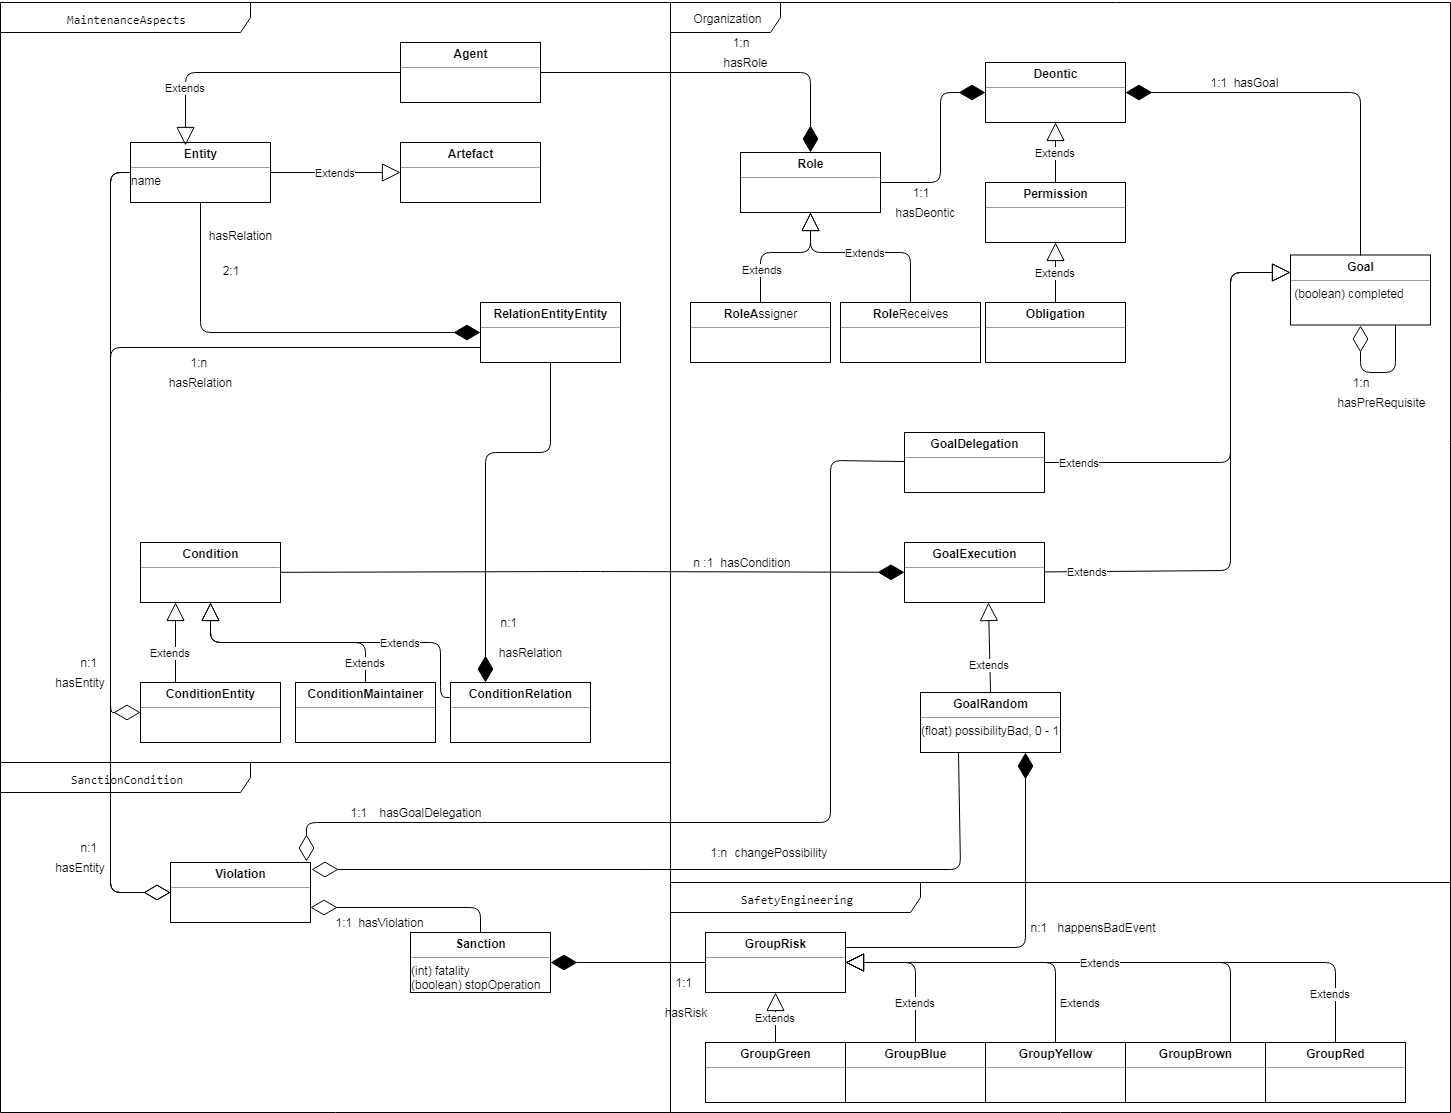
\includegraphics[width=0.8\linewidth]{umlmodel} 
\end{figure}

\end{document} 
